\vspace{-5pt}
\section{Introduction}
\label{sec:intro}
\vspace{-2pt}

With the rapid development of spatial computing, room reidentification (ReID) has become a key area of interest, enabling advancements in applications like augmented reality (AR) \cite{schult2023controlroom3droomgenerationusing} and homecare robotics \cite{sarch2022tideetidyingnovelrooms}. It plays a crucial role in enhancing user experiences across various scenarios. 
For instance, on devices like the Apple Vision Pro, accurate room ReID enables smooth transitions between virtual and real-world elements. 
% This includes adjusting workspace layouts and showing relevant information based on the current room. 
Similarly, in AR-guided museum tours, precisely identifying a user’s position within specific rooms is essential for delivering location-sensitive content.

\begin{figure}[ht]
    \centering
    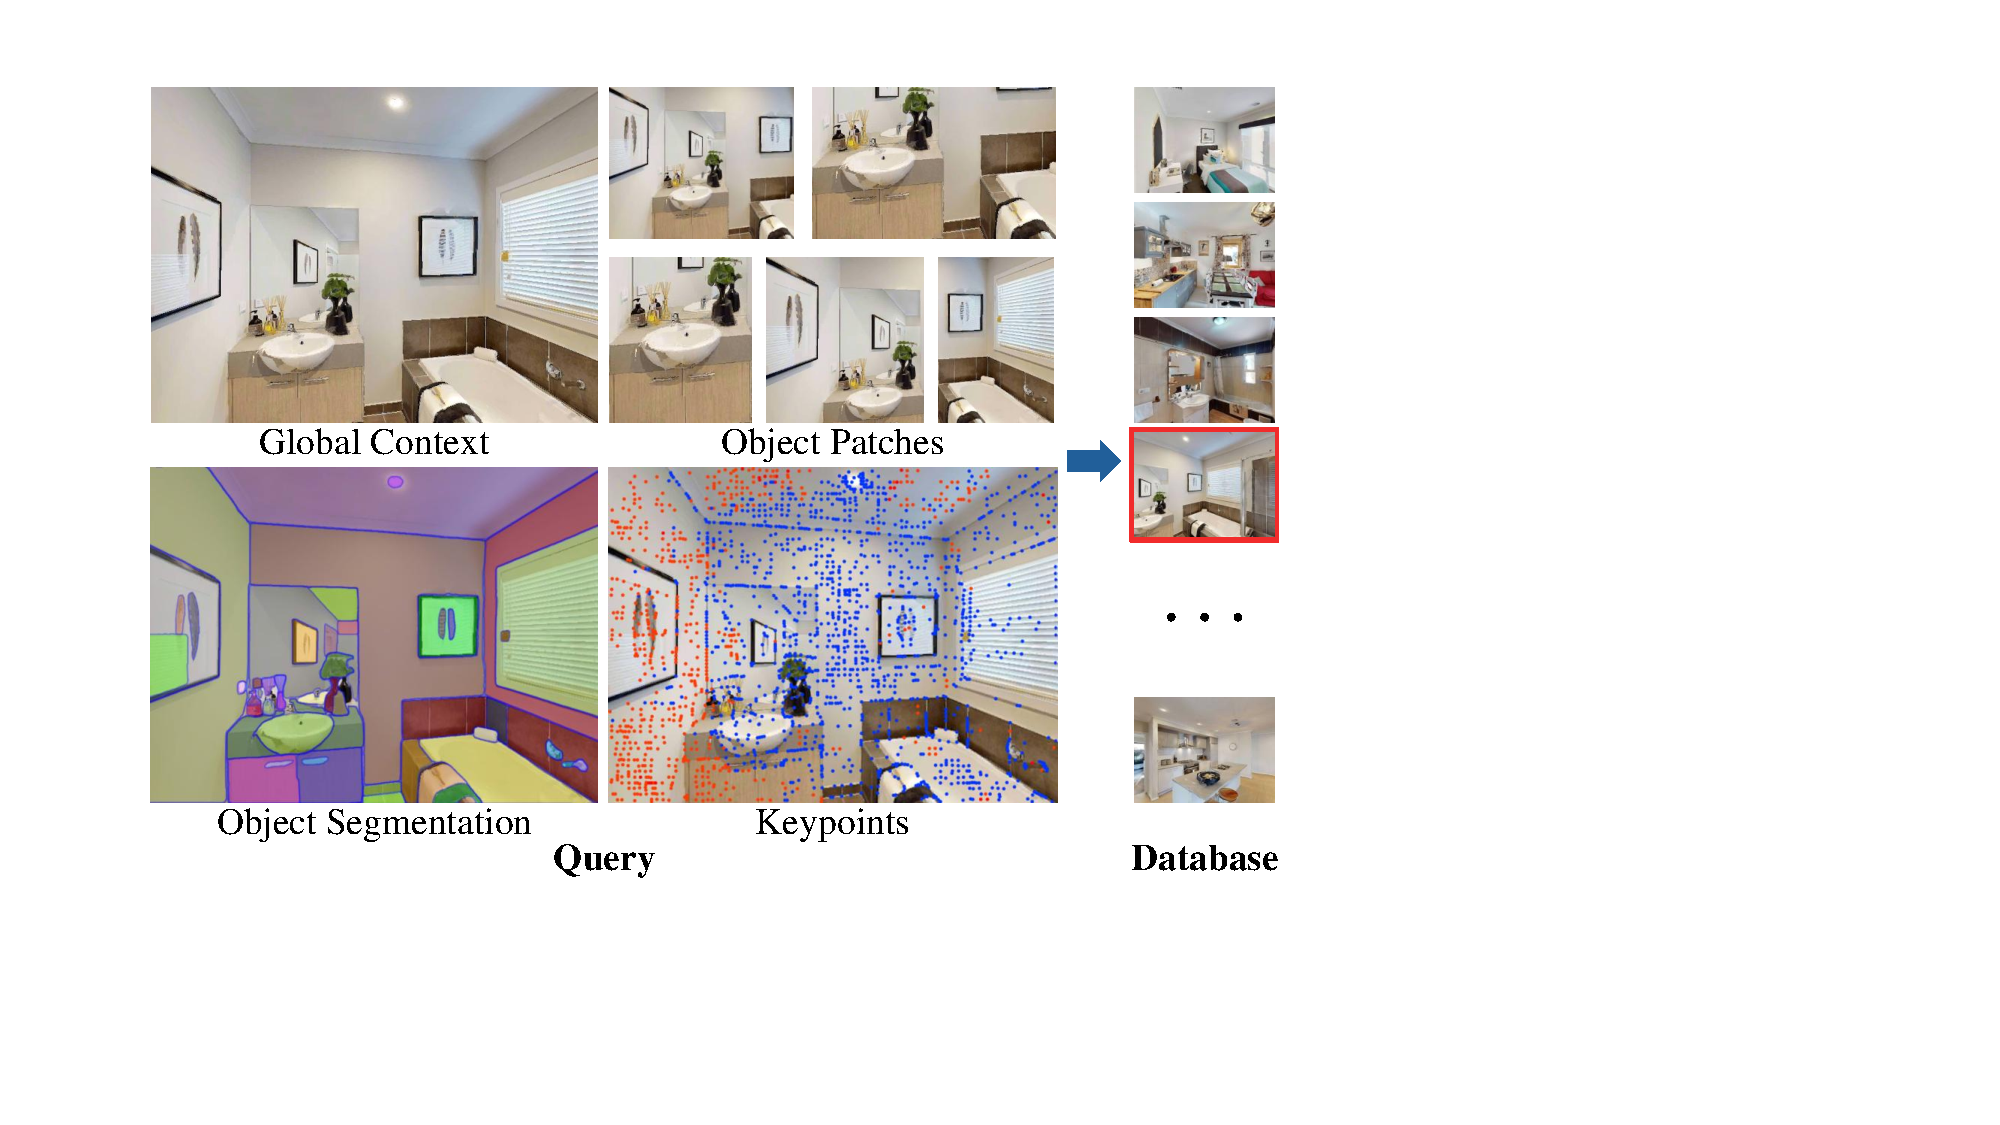
\includegraphics[width=\columnwidth]{object_information_font.pdf}
    \vspace{-20pt}
    \caption{AirRoom leverages multi-level, object-oriented features, including global context, object patches, object segmentation, and keypoints, to perform coarse-to-fine room reidentification.}
    \vspace{-20pt}
    \label{fig:example_image}
\end{figure}

Unlike outdoor environments, where visual place recognition (VPR) methods have matured and perform reliably \cite{arandjelović2016netvladcnnarchitectureweakly, hausler2021patchnetvladmultiscalefusionlocallyglobal, keetha2023anylocuniversalvisualplace}, indoor room ReID remains a challenging problem. A primary reason for this difficulty is the cluttered nature of indoor scenes, which are often densely packed with man-made objects \cite{xu2023clusvprefficientvisualplace}. These densely distributed objects often pose significant challenges to existing methods, which were originally designed for city-style and distinct structures \cite{7339473}. Consequently, these methods struggle to fully capture the intricate details and varied spatial layouts of indoor environments.
% , leading to limitations in their effectiveness when applied to densely populated indoor spaces.
For instance, foundation models like DINO \cite{caron2021emergingpropertiesselfsupervisedvision} and DINOv2 \cite{oquab2024dinov2learningrobustvisual} can generate global descriptors that capture broad scene-level features. However, these descriptors may struggle in semantically similar environments, such as adjacent rooms with similar layouts or decorations, where distinguishable features are minimal \cite{cai2022patchnetvladlearnedpatchdescriptor}. In contrast, methods like Patch-NetVLAD \cite{hausler2021patchnetvladmultiscalefusionlocallyglobal}, AirLoc \cite{aryan2023airlocobjectbasedindoorrelocalization} and AnyLoc \cite{keetha2023anylocuniversalvisualplace} create a global descriptor by aggregating local features, which can enhance discriminative power. Yet, in indoor settings densely populated with similar and repetitive objects, these approaches may still face difficulties in distinguishing between highly similar features, reducing their effectiveness in such contexts \cite{sattler2019understandinglimitationscnnbasedabsolute}.

Additionally, different from room categorization \cite{lee2017roomnetendtoendroomlayout}, which relies on identifying object types to classify spaces into semantic categories, 
%room ReID requires accurately matching specific room instances within a large pre-collected database.
room ReID requires accurately retrieving the same room instance from a reference database based on a given query image. 
For instance, reidentifying a particular kitchen demands a combination of global functional contexts and fine-grained matching of specific object attributes. Moreover, room ReID must handle viewpoint variations, which necessitates tolerance for partial mismatches in object arrangement and appearance. These requirements often result in the failure of algorithms based solely on object categorization, as they lack the precision needed to reidentify unique room instances accurately \cite{Snderhauf2015PlaceRW}.

This raises an important question: \textit{“What kinds of object attributes are truly essential for room ReID?”} To address this, we conduct the first comprehensive study exploring multi-level object-oriented information and its impact on room ReID.
As shown in \fref{fig:example_image}, our experiments show that all four levels of object-oriented information, \ie, global context, object patches, object segmentation, and keypoints, are essential.
Specifically, we find that each level plays a unique role in room ReID. Global context, such as the combination of objects like a couch and television, conveys essential semantic information for categorizing a room as a living room. Object patches provide finer details, enabling differentiation within a room, such as distinguishing a bedside table in a bedroom from a desk in a workspace. Object segmentation offers further granularity by isolating individual items, like separating a dining table from surrounding chairs to clarify the room layout. Finally, keypoints on objects, such as handles on a dresser, enhance room ReID by filtering out visually similar furniture in other rooms. Moreover, integrating multi-level object-oriented information adds robustness to viewpoint variations.

%To address this, we conduct the first comprehensive study that explores the impact of multi-level object information on room ReID. As shown in \fref{fig:example_image}, our experiments demonstrate that all four levels of object information, \textit{i.e.}, global context, object patches, object segmentation, and local keypoints, are essential. Specifically, we find that each level plays a unique role in room ReID. Global context, such as the combination of objects like a couch and television, provides semantic cues to classify a room as a living room. Object patches offer finer detail, helping to distinguish functional zones within a room, such as a sleeping area with a bed and nightstand or a makeup area with a mirror and dressing table in a bedroom. Object segmentation clarifies room layout by isolating specific items, like separating a dining table from surrounding chairs. Finally, local keypoints aid in identifying rooms by filtering out visually similar furniture in other spaces. Moreover, the integration of these four levels of object information significantly improves robustness to viewpoint variations, making our approach adaptable to diverse room perspectives.

% Recent approaches, such as AirLoc \cite{aryan2023airlocobjectbasedindoorrelocalization}, have begun to incorporate object information. However, they rely on pixel-aggregation to form object and room features, which sacrifices critical semantic information, resulting in suboptimal performance. Our findings indicate that objects within indoor environments inherently convey semantic information that aids in room categorization. For example, a combination of objects like a bed, bedside table, and dressing table strongly suggests a bedroom, rather than a kitchen. By incorporating global room representations enriched with object-derived semantics, we achieve broad categorization of rooms. Further, subsets of objects within a room can provide finer details, such as dividing a bedroom into zones like a rest area, with a bed and bedside table, and a makeup area, with a mirror and dressing table. These subsets, or “patches” in image terms, facilitate fine-grained candidate selection. Additionally, individual object details provide further refinement, and local feature matching enhances candidate filtering at an even finer level. Building on these insights, we propose AirRoom—a flexible, object-aware pipeline for room reidentification. AirRoom effectively leverages multi-level object information, boosting reidentification performance while adapting to various configurations, showcasing robustness and versatility across diverse scenarios.

% We find that indoor environments can be broadly categorized into functional types, such as offices, lobbies, and kitchens, each containing distinct semantic information due to the variety of objects present. 
% Global features, rich in appearance and semantic content and extracted from visual backbones, can help select a few functionally similar candidates from a larger pool of irrelevant options \cite{song2022supergfunifyinglocalglobal}. 
% Furthermore, even functionally similar rooms often contain varied objects; for example, different bathrooms may have unique sinks or bathtubs.
% Algorithms that capture this object-level information are generally more effective for achieving accurate and reliable indoor relocalization \cite{qiao2022objectsmatterlearningobject}. 
% Additionally, local feature matching methods, which preserve fine grid information, prove to be highly beneficial \cite{kuang2022densegapgraphstructureddensecorrespondence, wang2024efficientloftrsemidenselocal}. Building on these insights, we propose AirRoom, a novel and flexible object-aware pipeline for indoor relocalization. This approach effectively utilizes object encoding to enhance performance while adapting seamlessly to different module configurations, demonstrating robustness and versatility.
% Recently, methods like AirLoc \cite{aryan2023airlocobjectbasedindoorrelocalization} have attempted to incorporate object information; however, they typically derive object features through a pixel-aggregation approach. This emphasis on local rather than true object-level features has led to limited performance improvements.

% To address these limitations, we pose the question: \textbf{“What if we integrate object encoding into VPR methods?”} We find that indoor environments can be broadly categorized into functional types, such as offices, lobbies, and kitchens, each containing distinct semantic information due to the variety of objects present. Global features, rich in appearance and semantic content and extracted from visual backbones, can help select a few functionally similar candidates from a larger pool of irrelevant options \cite{song2022supergfunifyinglocalglobal}. Furthermore, even functionally similar rooms often contain varied objects; for example, different bathrooms may have unique sinks or bathtubs. Algorithms that capture this object-level information are generally more effective for achieving accurate and reliable indoor relocalization \cite{qiao2022objectsmatterlearningobject}. Additionally, local feature matching methods, which preserve fine grid information, prove to be highly beneficial \cite{kuang2022densegapgraphstructureddensecorrespondence, wang2024efficientloftrsemidenselocal}. Building on these insights, we propose ObjLoc, a novel and flexible object-aware pipeline for indoor relocalization. This approach effectively utilizes object encoding to enhance performance while adapting seamlessly to different module configurations, demonstrating robustness and versatility.
% Recently, methods like AirLoc \cite{aryan2023airlocobjectbasedindoorrelocalization} have attempted to incorporate object information; however, they typically derive object features through a pixel-aggregation approach. This emphasis on local rather than true object-level features has led to limited performance improvements.

Based on these observations, we propose AirRoom, a simple yet highly effective room reidentification (ReID) system consisting of three stages: Global, Local, and Fine-Grained. In the Global stage, a Global Feature Extractor is used to capture global context features, which are then employed to coarsely select five functionally similar candidate rooms. In the Local stage, instance segmentation is applied to identify individual objects, followed by the Receptive Field Expander to extract object patches. An Object Feature Extractor is then used to obtain both object and patch features, which are utilized in Object-Aware Scoring to narrow the selection down to two candidate rooms. Finally, in the Fine-Grained stage, feature matching is employed to precisely identify the final room.

In summary, our contributions include:

\begin{itemize}[leftmargin=2em]
    \item We introduce AirRoom, an object-aware room ReID pipeline with two novel modules: the Receptive Field Expander and Object-Aware Scoring, effectively leveraging multi-level object-oriented information to overcome the limitations observed in previous methods.
    \item We have curated four comprehensive room reidentification datasets—MPReID, HMReID, GibsonReID, and ReplicaReID—providing diverse benchmarks for evaluating room reidentification methods.
    \item Extensive experiments demonstrate that AirRoom outperforms SOTAs, maintaining robust and reliable performance even under significant viewpoint variations.
\end{itemize}
